\documentclass[a4paper]{article}

\usepackage[english]{babel}
\usepackage[utf8]{inputenc}
\usepackage{amsmath}
\usepackage{graphicx}
\usepackage{enumerate}
\usepackage{caption}
\usepackage[colorinlistoftodos]{todonotes}
\usepackage{graphicx}
\usepackage{advdate}
\usepackage{tikz}
\graphicspath{c:/Users/Max/Pictures}
\title{AE 370: Homework 5}

\author{Max A. Feinberg}

\date{\AdvanceDate[-1]\today}

\begin{document}
\maketitle

\section*{Problem 1}
Consider the beam bending problem shown below in Figure 1:

\begin{figure}[ht]
\centering
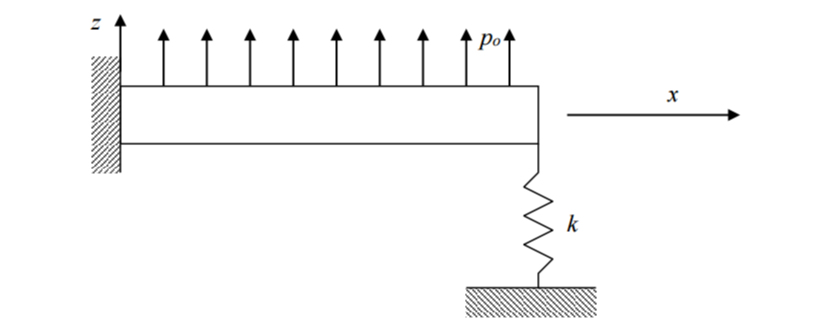
\includegraphics[scale=1.0]{AE370HW5.PNG}
\caption{A Beam Bending Problem}
\end{figure}
The potential energy of the system is defined by the following equation: 
\begin{eqnarray*}
\Pi & = & \frac{1}{2} \int_{0}^{L}EI\Big(\frac{d^{2}w}{dx^{2}}\Big)^{2} \ dx - \int_{0}^{L}\rho_{0}w \ dx + \frac{1}{2} k(w(L))^{2} 
\end{eqnarray*}
We also know the following boundary conditions:
\begin{eqnarray*}
w(0) & = & 0\\
\frac{dw}{dx}(0) & = & 0\\
\end{eqnarray*}
\textbf{1)} We will now use the Rayleigh-Ritz Method (RRM) to approximate the simplest solution to the problem.  We must begin with a second order polynomial because of the presence of a second derivative in the potential energy equation
\begin{eqnarray*}
\widetilde{w} & = & a_0 + a_{1}x + a_{2}x^{2}\\
\frac{d\tilde{w}}{dx} & = & a_{1} + 2a_{2}x\\
\frac{d^{2}\tilde{w}}{dx^{2}} & = & 2a_{2}\\
\end{eqnarray*}
When we apply the boundary conditions, we find the following:
\begin{eqnarray*}
\widetilde{w}(0) & = & a_0 + a_{1}x + a_{2}x^{2}\\
0 & = & a_{0}\\
\frac{d\tilde{w}}{dx} (0) & = & a_{1} + 2a_{2}x\\
0 & = & a_{1}\\
\end{eqnarray*}
This leaves us with the following equations:
\begin{eqnarray*}
\widetilde{w} & = & a_{2}x^{2}\\
\frac{d\tilde{w}}{dx} & = & 2a_{2}x\\
\frac{d^{2}\tilde{w}}{dx^{2}} & = & 2a_{2}\\
\end{eqnarray*}
Only one coefficient remains, so we will now refer to $a_{2}$ as $a$.  We will now substitute our approximation of the deflection equation into the energy equation.
\begin{eqnarray*}
\Pi & = & \frac{1}{2} \int_{0}^{L}EI(2a)^{2} \ dx - \int_{0}^{L}\rho_{0}(ax^{2}) \ dx + \frac{1}{2} k(aL^{2})^{2}\\
\Pi & = & 2EIa^{2}L-\frac{1}{3}\rho_{0}aL^{3} + \frac{1}{2}ka^{2}L^{4}
\end{eqnarray*} 
By applying the Principle of Minimum Potential Energy, we can determine the value of $a$.
\begin{eqnarray*}
\frac{d\Pi}{da} & = & 0\\
\frac{d\Pi}{da} & = & 4EIaL - \frac{1}{3}\rho_{0}L^{3} + kaL^{4}\\
\frac{1}{3}\rho_{0}L^{3} & = & a(4EIL + kL^{4})\\
a & = & \frac{\rho_{0}L}{3(4EIL+kL^{4})}\\
\end{eqnarray*}
This yields the following polynomial basis function:
\begin{eqnarray*}
EI\widetilde{w}(x) & = & \frac{EI\rho_{0}L}{3(4EIL+kL^{4})}x^{2}\\
\end{eqnarray*}
\textbf{2)}We will now find the approximation using one more polynomial term.
\begin{eqnarray*}
\widetilde{w} & = & a_0 + a_{1}x + a_{2}x^{2}+a_{3}x^{3}\\
\frac{d\tilde{w}}{dx} & = & a_{1} + 2a_{2}x + 3a_{3}x^{2}\\
\frac{d^{2}\tilde{w}}{dx^{2}} & = & 2a_{2} + 6a_{3}x\\
\end{eqnarray*}
Next, we will apply the boundary conditions:
\begin{eqnarray*}
\widetilde{w}(0) & = & a_0 + a_{1}x + a_{2}x^{2} + a_{3}x^{3}\\
0 & = & a_{0}\\
\frac{d\tilde{w}}{dx} (0) & = & a_{1} + 2a_{2}x + 3a_{3}x^{2}\\
0 & = & a_{1}\\
\end{eqnarray*}
This leaves us with the following equations:
\begin{eqnarray*}
\widetilde{w} & = & a_{2}x^{2} + a_{3}x^{3}\\
\frac{d\tilde{w}}{dx} & = & 2a_{2}x+3a_{3}x^{2}\\
\frac{d^{2}\tilde{w}}{dx^{2}} & = & 2a_{2} + 6a_{3}x\\
\end{eqnarray*}
To reduce confusion, we will now refer to $a_{2}$ as $a$ and $a_{3}$ as $b$.  We will now substitute our approximation of the deflection equation into the energy equation.
\begin{eqnarray*}
\Pi & = & \frac{1}{2} \int_{0}^{L}EI(2a+6bx)^{2} \ dx - \int_{0}^{L}\rho_{0}(ax^{2}+bx^{3}) \ dx + \frac{1}{2} k(aL^{2}+bL^{3})^{2}\\
\Pi & = & \frac{1}{2} \int_{0}^{L}EI(4a^{2}+24abx+36b^{2}x^{2}) \ dx - \int_{0}^{L}\rho_{0}(ax^{2}+bx^{3}) \ dx + \frac{1}{2} k(a^{2}L^{4}+2abL^{5}+b^{2}L^{6})\\
\Pi & = & 2EIa^{2}L+6EIabL^{2} + 6EIb^{2}L^{3}-\frac{1}{3}\rho_{0}aL^{3}-\frac{1}{4}\rho_{0}bL^{4}+\frac{1}{2}ka^{2}L^{4}+kabL^{5}+\frac{1}{2}kb^{2}L^{6}\\
\end{eqnarray*} 
By applying the Principle of Minimum Potential Energy, we can determine the value of $a$ and $b$.
\begin{eqnarray*}
\frac{d\Pi}{da} & = & 0\\
\frac{d\Pi}{da} & = & 4EIaL + 6EIbL^{2}- \frac{1}{3}\rho_{0}L^{3} + kaL^{4} + kbL^{5}\\
\frac{d\Pi}{da} & = & a(4EIL+kL^{4}) + b(6EIL^{2}+kL^{5}) - \frac{1}{3}\rho_{0}L^{3}\\
\frac{1}{3}\rho_{0}L^{3} & = & a(4EIL+kL^{4}) + b(6EIL^{2}+kL^{5}) \qquad (1)\\
\frac{d\Pi}{db} & = & 6EIaL^{2} + 12EIbL^{3}-\frac{1}{4}\rho_{0}L^{4}+kaL^{5}+kbL^{6}\\
\frac{d\Pi}{db} & = & a(6EIL^{2}+kL^{5})+b(12EIL^{3}+kL^{6}) -\frac{1}{4}\rho_{0}L^{4} \\
\frac{1}{4}\rho_{0}L^{4} & = & a(6EIL^{2}+kL^{5})+b(12EIL^{3}+kL^{6})  \quad (2)\\
\end{eqnarray*}
Using equation 1 and 2 above, we will now solve for a and b.
\begin{eqnarray*}
\begin{bmatrix}
4EIL+kL^{4} & 6EIL^{2} + kL^{5}\\
6EIL^{2}+kL^{5} & 12EIL^{3}+kL^{6}\\
\end{bmatrix}
\begin{bmatrix}
a \\ 
b
\end{bmatrix}
 & = & \begin{bmatrix}
\frac{1}{3}\rho_{0}L^{3}\\[3pt]
\frac{1}{4}\rho_{0}L^{4}
\end{bmatrix}\\
\end{eqnarray*}
\begin{eqnarray*}
\begin{bmatrix}
a\\
b
\end{bmatrix}
& = & 
\begin{bmatrix}
\frac{L^{2}\rho_{0}(30EI+kL^{3})}{48EI(3EI+kL^{3})}\\[3pt]
\frac{-L\rho_{0}(12EI+kL^{3})}{48EI(3EI+KL^{3})}
\end{bmatrix}
\end{eqnarray*}
This yields the following polynomial basis function:
\begin{eqnarray*}
EI\widetilde{w}(x) & = & \frac{EIL^{2}\rho_{0}(30EI+kL^{3})}{48EI(3EI+kL^{3})}x^{2} + \frac{-EIL\rho_{0}(12EI+kL^{3})}{48EI(3EI+KL^{3})}x^{3} \\
EI\widetilde{w}(x) & = & \frac{L^{2}\rho_{0}(30EI+kL^{3})}{48(3EI+kL^{3})}x^{2} + \frac{-L\rho_{0}(12EI+kL^{3})}{48(3EI+KL^{3})}x^{3} \\
EI\widetilde{w}(x) & = & \frac{L\rho_{0}}{48EI(3EI+KL^{3})}x^{2}((30EI+kL^{3})-(12EI+kL^{3})x)\\
\end{eqnarray*}

\pagebreak

\begin{figure}[ht]
\centering
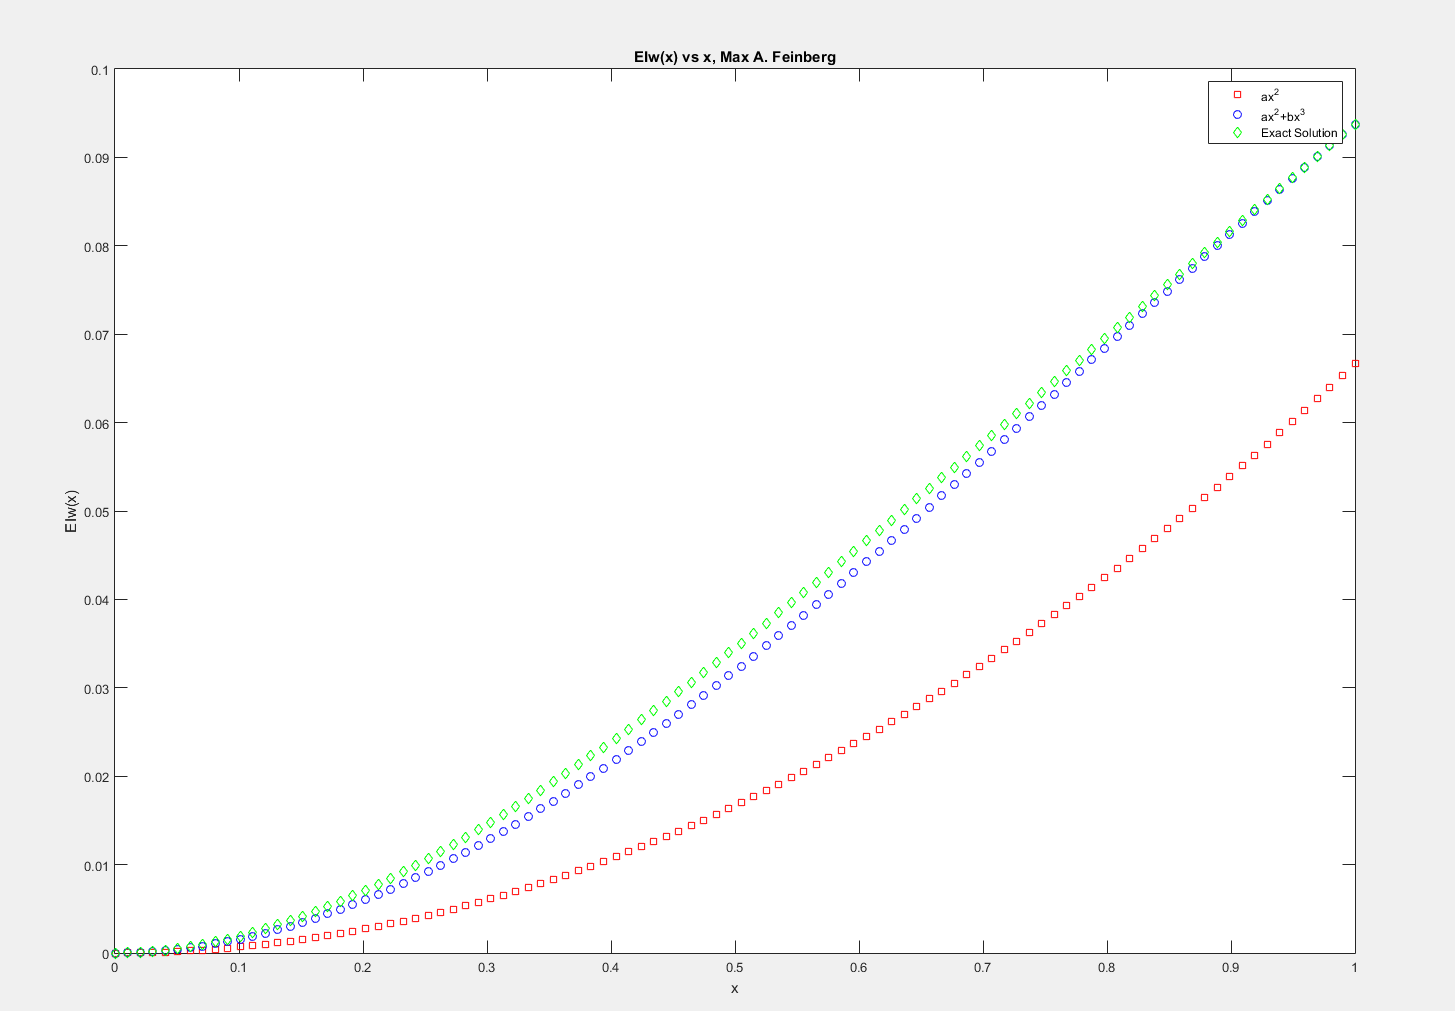
\includegraphics[scale=
.35]{AE370HW5convergence.PNG}
\caption{A graph showing the convergence of the RRM approximations found above and the exact solutions}
\end{figure}

As it can be clearly seen in Figure 2 above, the cubic polynomial basis function approximation that was found via the RRM closely estimates the actual solutions.

\pagebreak

\section*{Problem 2}

Consider the bi-material axially loaded bar structure of length 2L defined below in Figure 3:

\begin{figure}[ht]
\centering
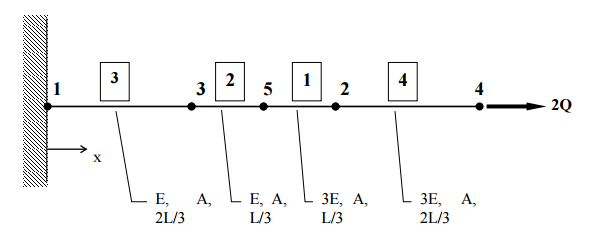
\includegraphics[scale=1.0]{AE370HWP2.PNG}
\caption{A Beam Bending Problem}
\end{figure}

The potential energy equations for each section shall be defined as follows:
\begin{eqnarray*}
\Pi & = & \frac{1}{2} \langle U_{a} \ U_{b} \rangle \left\{  k \right \}  \begin{bmatrix}
U_{a} \\ 
U_{b}
\end{bmatrix} - \langle U_{a} \ U_{b} \rangle \{ r \} \\
\{ k \}
& = &
\frac{EA}{L}
\begin{bmatrix}
1 & -1 \\
-1 & 1
\end{bmatrix}\\
\{ r \} & = &
\rho_{0}L 
\begin{bmatrix}
1/2 \\
1/2
\end{bmatrix}\\
\rho & = & \rho_{0}\Big(\frac{x}{2L}\Big)^{2}\\
\end{eqnarray*}
Where $a$ and $b$ are defined as the beginning and ending nodes for the element that is currently being analyzed.\\
$$a = 1, \ b = 3, \ EA, \ l = \frac{2}{3}L, \rho = \rho_{0}\Big(\frac{\frac{L}{3}}{2L}\Big)^{2} = \rho_{0}\Big(\frac{1}{6}\Big)^{2}$$
\begin{eqnarray*}
\Pi^{(3)} & = & \frac{1}{2} \langle U_{1} \ U_{3} \rangle \frac{EA}{\frac{2L}{3}}
\begin{bmatrix}
1 & -1 \\
-1 & 1
\end{bmatrix}  \begin{bmatrix}
U_{1} \\ 
U_{3}
\end{bmatrix} - \langle U_{1} \ U_{3} \rangle \rho_{0}\frac{2L}{3} 
\begin{bmatrix}
\frac{1}{2}\Big(\frac{1}{6}\Big)^{2} \\
\frac{1}{2}\Big(\frac{1}{6}\Big)^{2}
\end{bmatrix} \\
\end{eqnarray*}
\pagebreak
$$a = 3, \ b = 5, \ EA, \ l = \frac{L}{3}, \rho = \rho_{0}\Big(\frac{\frac{5L}{6}}{2L}\Big)^{2} = \rho_{0}\Big(\frac{5}{12}\Big)^{2}$$
\begin{eqnarray*}
\Pi^{(2)} & = & \frac{1}{2} \langle U_{3} \ U_{5} \rangle \frac{EA}{\frac{L}{3}}
\begin{bmatrix}
1 & -1 \\
-1 & 1
\end{bmatrix}  \begin{bmatrix}
U_{3} \\ 
U_{5}
\end{bmatrix} - \langle U_{3} \ U_{5} \rangle \rho_{0}\frac{L}{3} 
\begin{bmatrix}
\frac{1}{2}\Big(\frac{5}{12}\Big)^{2} \\
\frac{1}{2}\Big(\frac{5}{12}\Big)^{2}
\end{bmatrix} \\
\end{eqnarray*}
$$a = 5, \ b = 2, \ 3EA, \ l = \frac{L}{3}, \rho = \rho_{0}\Big(\frac{\frac{7L}{6}}{2L}\Big)^{2} = \rho_{0}\Big(\frac{7}{12}\Big)^{2}$$
\begin{eqnarray*}
\Pi^{(1)} & = & \frac{1}{2} \langle U_{5} \ U_{2} \rangle \frac{3EA}{\frac{L}{3}}
\begin{bmatrix}
1 & -1 \\
-1 & 1
\end{bmatrix}  \begin{bmatrix}
U_{5} \\ 
U_{2}
\end{bmatrix} - \langle U_{5} \ U_{2} \rangle \rho_{0}\frac{L}{3} 
\begin{bmatrix}
\frac{1}{2}\Big(\frac{7}{12}\Big)^{2} \\
\frac{1}{2}\Big(\frac{7}{12}\Big)^{2}
\end{bmatrix} \\
\end{eqnarray*}
$$a = 2, \ b = 4, \ 3EA, \ l = \frac{2L}{3}, \rho = \rho_{0}\Big(\frac{\frac{5L}{3}}{2L}\Big)^{2} = \rho_{0}\Big(\frac{5}{6}\Big)^{2}$$
\begin{eqnarray*}
\Pi^{(4)} & = & \frac{1}{2} \langle U_{2} \ U_{4} \rangle \frac{3EA}{\frac{2L}{3}}
\begin{bmatrix}
1 & -1 \\
-1 & 1
\end{bmatrix}  \begin{bmatrix}
U_{2} \\ 
U_{4}
\end{bmatrix} - \langle U_{2} \ U_{4} \rangle \rho_{0}\frac{2L}{3} 
\begin{bmatrix}
\frac{1}{2}\Big(\frac{5}{6}\Big)^{2} \\
\frac{1}{2}\Big(\frac{5}{6}\Big)^{2}
\end{bmatrix} \\
\end{eqnarray*}
Using the equations for each element defined above, we will construct the global energy equation.
\begin{eqnarray*}
\Pi^{Total} & = & \frac{1}{2}\langle U_{1} \ U_{2} \ U_{3} \ U_{4} \ U_{5} \rangle \frac{EA}{L} \begin{bmatrix}
\frac{3}{2} & 0 & -\frac{3}{2} & 0 & 0 \\
0 & 9 + \frac{9}{2} & 0 & -\frac{9}{2} & -9\\
-\frac{3}{2} & 0 & \frac{3}{2} + 3 & 0 & -3\\
0 & -\frac{9}{2} & 0 & \frac{9}{2} & 0\\
0 & -9 & -3 & 0 & 9 +3\\
\end{bmatrix}
\begin{bmatrix}
U_{1}\\
U_{2}\\
U_{3}\\
U_{4}\\
U_{5}\\
\end{bmatrix}\\
& & - \langle U_{1} \ U_{2} \ U_{3} \ U_{4} \ U_{5} \rangle
\rho_{0}L
\begin{bmatrix}
\frac{1}{3} \big( \frac{1}{6}\big)^{2}\\[3pt]
\frac{1}{6} \big(\frac{7}{12} \big)^{2}+\frac{1}{3} \big(\frac{5}{6}\big)^{2}\\[3pt]
\frac{1}{3} \big(\frac{1}{6} \big)^{2}+\frac{1}{6} \big(\frac{5}{12}\big)^{2}\\[3pt]
\frac{1}{3} \big( \frac{5}{6}\big)^{2}\\[3pt]
\frac{1}{6} \big(\frac{7}{12} \big)^{2}+\frac{1}{6} \big(\frac{5}{12}\big)^{2}\\
\end{bmatrix}
\end{eqnarray*}
Node 1 is fixed so we can reduce our equation to the following.
\begin{eqnarray*}
\Pi^{Total} & = & \frac{1}{2}\langle U_{2} \ U_{3} \ U_{4} \ U_{5} \rangle \frac{EA}{L} 
\begin{bmatrix}
9 + \frac{9}{2} & 0 & -\frac{9}{2} & -9\\
0 & \frac{3}{2} + 3 & 0 & -3\\
-\frac{9}{2} & 0 & \frac{9}{2} & 0\\
-9 & -3 & 0 & 9 +3\\
\end{bmatrix}
\begin{bmatrix}
U_{2}\\
U_{3}\\
U_{4}\\
U_{5}\\
\end{bmatrix}\\
& & - \langle U_{2} \ U_{3} \ U_{4} \ U_{5} \rangle
\rho_{0}L
\begin{bmatrix}
\frac{1}{6} \big(\frac{7}{12} \big)^{2}+\frac{1}{3} \big(\frac{5}{6}\big)^{2}\\[3pt]
\frac{1}{3} \big(\frac{1}{6} \big)^{2}+\frac{1}{6} \big(\frac{5}{12}\big)^{2}\\[3pt]
\frac{1}{3} \big( \frac{5}{6}\big)^{2}\\[3pt]
\frac{1}{6} \big(\frac{7}{12} \big)^{2}+\frac{1}{6} \big(\frac{5}{12}\big)^{2}\\
\end{bmatrix}
\end{eqnarray*}
We can now consider the final linear equation:
\begin{eqnarray*}
\{k \} \{ u \} & = & \{ r \} + \{ Q \}\\
\begin{bmatrix}
9 + \frac{9}{2} & 0 & -\frac{9}{2} & -9\\
0 & \frac{3}{2} + 3 & 0 & -3\\
-\frac{9}{2} & 0 & \frac{9}{2} & 0\\
-9 & -3 & 0 & 9 +3\\
\end{bmatrix}
\begin{bmatrix}
U_{2}\\
U_{3}\\
U_{4}\\
U_{5}\\
\end{bmatrix}
& = & 
\begin{bmatrix}
\frac{1}{6} \big(\frac{7}{12} \big)^{2}+\frac{1}{3} \big(\frac{5}{6}\big)^{2}\\[3pt]
\frac{1}{3} \big(\frac{1}{6} \big)^{2}+\frac{1}{6} \big(\frac{5}{12}\big)^{2}\\[3pt]
\frac{1}{3} \big( \frac{5}{6}\big)^{2}\\[3pt]
\frac{1}{6} \big(\frac{7}{12} \big)^{2}+\frac{1}{6} \big(\frac{5}{12}\big)^{2}\\
\end{bmatrix} +
\begin{bmatrix}
0\\
0\\
2Q\\
0\\
\end{bmatrix}\\
\begin{bmatrix}
9 + \frac{9}{2} & 0 & -\frac{9}{2} & -9\\
0 & \frac{3}{2} + 3 & 0 & -3\\
-\frac{9}{2} & 0 & \frac{9}{2} & 0\\
-9 & -3 & 0 & 9 +3\\
\end{bmatrix}
\begin{bmatrix}
U_{2}\\
U_{3}\\
U_{4}\\
U_{5}\\
\end{bmatrix}
& = & 
\begin{bmatrix}
\frac{1}{6} \big(\frac{7}{12} \big)^{2}+\frac{1}{3} \big(\frac{5}{6}\big)^{2}\\[3pt]
\frac{1}{3} \big(\frac{1}{6} \big)^{2}+\frac{1}{6} \big(\frac{5}{12}\big)^{2}\\[3pt]
\frac{1}{3} \big( \frac{5}{6}\big)^{2} + 2Q\\[3pt]
\frac{1}{6} \big(\frac{7}{12} \big)^{2}+\frac{1}{6} \big(\frac{5}{12}\big)^{2}\\
\end{bmatrix}
\end{eqnarray*}
In element 2, the stress, $\sigma_{2}$, can be found via the equation $\sigma_{2} = E \frac{\Delta L_{53}}{\frac{L}{3}}$ where $\Delta L_{53}$ is defined as the change in displacement of nodes 5 and 3. Similarly, the stress in element 4, $\sigma_{4}$, can be found via the equation $\sigma_{4} = E \frac{\Delta L_{42}}{\frac{2L}{3}}$ where $\Delta L_{42}$ is defined as the change in displacement of nodes 4 and 2.

\section*{Problem 3}

\begin{figure}[ht]
\centering
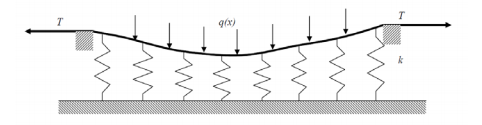
\includegraphics[scale=
.75]{AE370HW3P3.PNG}
\caption{A string of length L under tension T that is subjected to a transverse load $q(x)$ and lies above a distributed elastic foundation}
\end{figure}

Let the energy of the system shown above in Figure 4 be defined as follows:
\begin{eqnarray*}
\Pi & = & \frac{1}{2}\int_{0}^{L} \Big\{T\Big( \frac{dw}{dx}\Big)^{2} kw^{2} \Big\} \ dx - \int_{0}^{L}q_{0} w(x) \ dx\\
\end{eqnarray*}
We will split the string into 3 2-noded elements of length $\frac{L}{3}$. \\
\begin{center}
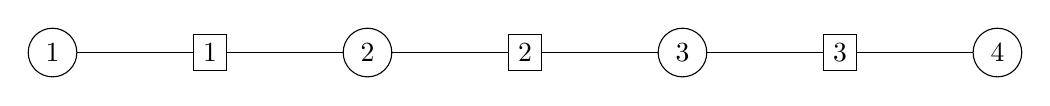
\begin{tikzpicture}
                \node[shape=circle, draw=black] (A) at (0, 0) {$1$};
                \node[shape=circle, draw=black] (B) at (4, 0) {$2$};
                \node[shape=circle, draw=black] (C) at (8, 0) {$3$};
                \node[shape=circle, draw=black] (D) at (12, 0) {$4$};
                 \node[shape=rectangle, draw=black] (E) at (2, 0) {$1$};
                 \node[shape=rectangle, draw=black] (F) at (6, 0) {$2$};
                 \node[shape=rectangle, draw=black] (G) at (10, 0) {$3$};
                \path[-] (A) edge node[] {} (E);
                \path[-] (E) edge node[] {} (B);
                \path[-] (B) edge node[] {} (F);
                \path[-] (F) edge node[] {} (C);
                \path[-] (C) edge node[] {} (G);
                \path[-] (G) edge node[] {} (D);
\end{tikzpicture}\\
\end{center}
In the diagram above, the number in circles denote nodes, and the numbers in rectangles denote elements.\\
Let us define the following shape functions: 
$$N_{1}(s)  =  1 - \frac{s}{L}, \
N_{2}(s)  =  \frac{s}{L}$$
We can now consider the deflection approximation equation:
$$\widetilde{w}(s) = N_{1}(s)W_{1}+N_{2}(s)W_{2} = \langle N_{1}(s) \ N_{2}(s) \rangle \begin{bmatrix}
W_{1}\\
W_{2}
\end{bmatrix} = \langle W_{1} \ W_{2} \rangle \begin{bmatrix}
N_{1}(s)\\
N_{2}(s)
\end{bmatrix}$$
To simplify this expression, we will also use the following notation:
$$\widetilde{w}(s) = \langle N \rangle \{ d \} = \langle N \rangle \{ d \}$$
We will define our potential energy functions for each elements as follows:
\begin{eqnarray*}
\Pi^{(e)} & = & \frac{1}{2} \int_{0}^{L} \Big\{T(\widetilde{w}')^{2} + k \widetilde{w}^{2} \Big\} \ ds - \int_{0}^{L}q_{0}\widetilde{w} \ ds\\
\Pi^{(e)} & = & \frac{1}{2} \int_{0}^{L} \Big\{T(W_{1}^{2}\Big(\frac{d N_{1}}{ds}\Big)^{2}+W_{1}W_{2}\frac{d N_{1}}{ds}\frac{d N_{2}}{ds} + W_{2}^{2}\Big(\frac{d N_{2}}{ds}\Big)^{2}) \Big\} \ ds \\
& & + \int_{0}^{L} k (W_{1}^{2}N^{2}_{1}(s) + 2 W_{1}W_{2}N_{1}(s)N_{2}(s) + W_{2}^{2}N_{2}^{2}(s)) \ ds \\
& & -
\int_{0}^{L}q_{0}(W_{1}N_{1}(s)+W_{2}N_{2}(s)) \ ds\\
\Pi^{(e)} & = &
\frac{1}{2} \langle W_{1} \ W_{2}\rangle
\begin{bmatrix}
\int_{0}^{L}T\Big(\frac{dN_{1}}{ds} \Big)^{2} + kN_{1}^{2}(s) \ ds & \int_{0}^{L}T\Big(\frac{dN_{1}}{ds} \Big)\Big(\frac{dN_{2}}{ds} \Big) + kN_{1}(s)N_{2}(s) \ ds \\
\int_{0}^{L}T\Big(\frac{dN_{1}}{ds} \Big)\Big(\frac{dN_{2}}{ds} \Big) + kN_{1}(s)N_{2}(s) \ ds & 
\int_{0}^{L}T\Big(\frac{dN_{2}}{ds} \Big)^{2} + kN_{2}^{2}(s) \ ds
\end{bmatrix}
\begin{bmatrix}
W_{1}\\
W_{2}
\end{bmatrix}\\
& & - \langle W_{1} \ W_{2} \rangle 
\begin{bmatrix}
\int_{0}^{L}q_{0}N_{1}(s) \ ds\\[3pt]
\int_{0}^{L}q_{0}N_{2}(s) \ ds\\
\end{bmatrix}\\
\Pi^{(e)} & = & \frac{1}{2}\langle W_{1} \ W_{2} \rangle \begin{bmatrix}
k
\end{bmatrix} 
\begin{bmatrix}
W_{1} \\ W_{2}
\end{bmatrix} - \langle W_{1} \ W_{2} \rangle \{ r \} \\
\end{eqnarray*}
The matrix k is the local stiffness matrix and r is the local load vector. With this simplified matrix form, we will find the potential equations for each element.
\begin{eqnarray*}
\Pi^{(1)} & = &
\frac{1}{2} \langle W_{1} \ W_{2}\rangle
\begin{bmatrix}
\int_{0}^{L}\frac{T}{L^{2}} + k(1 - \frac{2s}{L} + \frac{s^{2}}{L^{2}}) \ ds & \int_{0}^{L}-\frac{T}{L^{2}} + k(\frac{s}{L}-\frac{s^{2}}{L^{2}}) \ ds \\[3pt]
\int_{0}^{L}-\frac{T}{L^{2}} + k(\frac{s}{L}-\frac{s^{2}}{L^{2}}) \ ds & 
\int_{0}^{L}\frac{T}{L^{2}} + k(1 - \frac{2s}{L} + \frac{s^{2}}{L^{2}}) \ ds
\end{bmatrix}
\begin{bmatrix}
W_{1}\\
W_{2}
\end{bmatrix}\\
& & - \langle W_{1} \ W_{2} \rangle 
\begin{bmatrix}
\int_{0}^{L}q_{0}-\frac{q_{0}s}{L} \ ds\\
\int_{0}^{L}\frac{q_{0}s}{L} \ ds\\
\end{bmatrix}\\
\Pi^{(1)} & = & \frac{1}{2} \langle W_{1} \ W_{2} \rangle \begin{bmatrix}
\frac{3T}{L}+\frac{kL}{9} & -\frac{3T}{L}+ \frac{kL}{18}\\[3pt]
-\frac{3T}{L} + \frac{kL}{18} & 
\frac{3T}{L} + \frac{kL}{9}\\
\end{bmatrix}
\begin{bmatrix}
W_{1}\\
W_{2}\\
\end{bmatrix}
- \langle W_{1} \ W_{2} \rangle \begin{bmatrix}
\frac{q_{0}L}{6}\\
\frac{q_{0}L}{6}\\
\end{bmatrix}
\end{eqnarray*}
By symmetry we can also quickly find the potential equations for elements 2 and 3.
\begin{eqnarray*}
\Pi^{(2)} & = & \frac{1}{2} \langle W_{2} \ W_{3} \rangle \begin{bmatrix}
\frac{3T}{L}+\frac{kL}{9} & -\frac{3T}{L}+ \frac{kL}{18}\\[3pt]
-\frac{3T}{L} + \frac{kL}{18} & 
\frac{3T}{L} + \frac{kL}{9}\\
\end{bmatrix}
\begin{bmatrix}
W_{2}\\
W_{3}\\
\end{bmatrix}
- \langle W_{2} \ W_{3} \rangle \begin{bmatrix}
\frac{q_{0}L}{6}\\
\frac{q_{0}L}{6}\\
\end{bmatrix}
\end{eqnarray*}
\begin{eqnarray*}
\Pi^{(3)} & = & \frac{1}{2} \langle W_{3} \ W_{4} \rangle \begin{bmatrix}
\frac{3T}{L}+\frac{kL}{9} & -\frac{3T}{L}+ \frac{kL}{18}\\[3pt]
-\frac{3T}{L} + \frac{kL}{18} & 
\frac{3T}{L} + \frac{kL}{9}\\
\end{bmatrix}
\begin{bmatrix}
W_{3}\\
W_{4}\\
\end{bmatrix}
- \langle W_{3} \ W_{4} \rangle \begin{bmatrix}
\frac{q_{0}L}{6}\\
\frac{q_{0}L}{6}\\
\end{bmatrix}
\end{eqnarray*}
We will now construct the global stiffness matrix and the global load vector for $\Pi^{Total}$.
\begin{eqnarray*}
\begin{bmatrix}
k
\end{bmatrix} & = & \frac{T}{L}
\begin{bmatrix}
3 & -3 & 0 & 0\\
-3 & 6 & -3 & 0\\
0 & -3 & 6 & -3\\
0 & 0 & -3 & 3\\
\end{bmatrix} +
kL
\begin{bmatrix}
\frac{1}{9} & \frac{1}{18} & 0 & 0 \\[3pt]
\frac{1}{18} & \frac{2}{9} & \frac{1}{18} & 0 \\[3pt]
0 & \frac{1}{18} & \frac{2}{9} & \frac{1}{18} \\[3pt]
0 & 0 & \frac{1}{18} & \frac{1}{9} \\[3pt]
\end{bmatrix}\\
\{r\} & = & q_{0}L
\begin{bmatrix}
\frac{1}{6} \\[3pt]
\frac{1}{3} \\[3pt]
\frac{1}{3} \\[3pt]
\frac{1}{6} \\[3pt]
\end{bmatrix}
\end{eqnarray*}
By applying the boundary conditions, we can simplify our matrices as nodes 1 and 4 are fixed.
\begin{eqnarray*}
\begin{bmatrix}
k
\end{bmatrix} & = & \frac{T}{L}
\begin{bmatrix}
3 & -3 & 0 & 0\\
-3 & 6 & -3 & 0\\
0 & -3 & 6 & -3\\
0 & 0 & -3 & 3\\
\end{bmatrix} +
kL
\begin{bmatrix}
\frac{1}{9} & \frac{1}{18} & 0 & 0 \\[3pt]
\frac{1}{18} & \frac{2}{9} & \frac{1}{18} & 0 \\[3pt]
0 & \frac{1}{18} & \frac{2}{9} & \frac{1}{18} \\[3pt]
0 & 0 & \frac{1}{18} & \frac{1}{9} \\[3pt]
\end{bmatrix}\\
\{ r \} + \{ T \} & = &
q_{0}L
\begin{bmatrix}
\frac{1}{6} \\[3pt]
\frac{1}{3} \\[3pt]
\frac{1}{3} \\[3pt]
\frac{1}{6} \\[3pt]
\end{bmatrix}
+ 
\begin{bmatrix}
-T \\[3pt]
0 \\[3pt]
0 \\[3pt]
T \\[3pt]
\end{bmatrix}\\
\begin{bmatrix}
k
\end{bmatrix} & = & \frac{T}{L}
\begin{bmatrix}
 6 & -3\\
 -3 & 6\\
\end{bmatrix} +
kL
\begin{bmatrix}
\frac{2}{9} & \frac{1}{18}\\[3pt]
\frac{1}{18} & \frac{2}{9}\\[3pt]
\end{bmatrix}\\
\{ r \} + \{ T \} & = &
q_{0}L
\begin{bmatrix}
\frac{1}{3} \\[3pt]
\frac{1}{3} \\[3pt]
\end{bmatrix}
+ 
\begin{bmatrix}
0 \\[3pt]
0 \\[3pt]
\end{bmatrix}
\end{eqnarray*}
These leaves us with the following final matrix equation.
\begin{eqnarray*}
\Big\{ 
\frac{T}{L}
\begin{bmatrix}
 6 & -3\\
 -3 & 6\\
\end{bmatrix} +
kL
\begin{bmatrix}
\frac{2}{9} & \frac{1}{18}\\[3pt]
\frac{1}{18} & \frac{2}{9}\\[3pt]
\end{bmatrix}
\Big\}
\begin{bmatrix}
W_{2} \\
W_{3} \\ 
\end{bmatrix}
& = &
q_{0}L
\begin{bmatrix}
\frac{1}{3} \\[3pt]
\frac{1}{3} \\[3pt]
\end{bmatrix}\\
\end{eqnarray*}
By solving this equation, we find the following result:
$$W_{2} = W_{3} = \frac{6q_{0}L^{2}}{54T+5kL^{2}}$$
This result makes sense when compared to the physical situation as using stiffer springs or increasing the tension on the string should decrease the deflection.  As the transverse load increases, logically the deflection should increase as it does in our derived equation.
\end{document}